\section{Tools and Methodologies}
Traditionally, applications for trusted personal devices undergo
extensive testing and code review in order to avoid programming 
errors and security flaws. However, test campaigns and code review
can be expensive and do not guarantee the absence of programming
errors and security flaws. Thus, we propose to use validation
techniques based on annotations and verification conditions,
that do guarantee the lack of programming mistakes and that
all security properties that have been specified and verified
do indeed hold.



This chapter describes some tools that have been developed during the
Inspired project, that can be handled to validate Java applications
and methodologies that can be applied depending on different
validation purposes.  All those tools are part a Java application
validation workshop called JACK.


The first section is a general presentation of the JACK tool, section
2 introduces a JACK extension allowing to verify with some automation
some security properties, section 3 presents an associated tool
allowing to describe security properties with automata, section 4 is
about the proof facilities in JACK, section 5 describes Jack features
at bytecode level and section 6 concludes with some perspectives in
Java application validation tool development.

\subsection{JACK}
This section presents the Java Applet Correctness Kit (or \JACK).
This tool, already briefly described in \cite{BRL-JACK}, is
a formal tool that allows one to prove properties on Java programs
using the Java Modeling Language \cite{Leavens-Baker-Ruby03} (JML).
It has been developed initially by Gemplus, and since 2003 by INRIA
in the context of a bilateral collaboration with Gemplus, and then
in the context of the INSPIRED project.


It generates proof obligations allowing to prove that the Java code
conforms to its JML specification.  The lemmas are translated into an
internal formula language called JPOL (Java/Jack Proof Obligation
Language). Then JPOL verification conditions are translated into
different prover language, namely Coq, PVS, Simplify and the B
language \cite{bbook}, allowing to use the automatic provers Simplify
and the provers developed within the B method and interactive provers
like the Coq proof assistant, PVS or Click'n'Prove.

 But the tool is not yet another lemma generator for Java, since it
 also provides a lemma viewer integrated in the eclipse
 IDE\footnote{\texttt{http://www.eclipse.org}}, which is one of the
 most commonly used IDE for Java developers.  This allows to hide the
 formalisms used behind a graphical interface.  Lemmas are presented
 to users in a way they can understand them easier, by using the Java
 syntax and highlighting code portions to help the
 understanding. Using \JACK, one does not have to learn a formal
 language to be confident on code correctness.

\subsubsection{Jack Proof Obligation Language}
 \label{JPOL}
The Java/Jack Proof Obligation Language is an internal language used in Jack to represent verification conditions issued from the weakest precondition calculus. It can be considered as a melting-pot language based on first order logic with some specific features like:
\begin{itemize}
\item some basic set theory constructions (coming from the B notation)
\item some JML keywords
\item some Java constructions
\end{itemize}
The language is typed but has no specific syntax. It corresponds to an internal representation in the tool. Its semantic is given by the translation into the different theorem provers. Adding a theorem prover in JACK corresponds mainly to convert expressions of the JPOL language into the specific theorem prover language.

\subsubsection{JACK Plugins}

\subsection{Security property propagation}\label{sec:highlevel}

While JML is easily accessible to Java developers and tools exist
to manage the annotations, actually writing
the specifications of a Java application is labor-intensive and
error-prone, as it is easy to forget some annotations. There
exist tools which assist in writing these annotations,
\emph{e.g.}~Daikon~\cite{ErnstCGN2001:TSE} and Houdini~\cite{FlanaganL01}
use heuristic methods to produce annotations for simple safety and
functional invariants.  However, these tools cannot be guided by the
user---they do not require any user input---and in particular cannot
be used to synthesize annotations from realistic security policies.

We describe here, a method that, given a security policy,
automatically annotates a Java (Card) application, in such a way that
if the application respects the annotations then it also respects the
security policy. The generation of annotations proceeds in two phases:
synthesizing and weaving.
\begin{enumerate}
\item Based on the security policy we \emph{synthesize} core annotations, 
specifying the behavior of the methods directly involved.
\item Next we propagate these annotations to all methods directly or
indirectly invoking the methods that form the core of the security
policy, thus \emph{weaving} the security policy throughout the
application. 
\end{enumerate} 
This section is organized as follows. Subsection~\ref{SecHighLevelSecProp}
introduces several typical high-level security properties. Next,
Subsection~\ref{SecVerif} presents the process to weave these properties
throughout applications.


To show the usefulness of our approach, we applied the algorithm to
several realistic examples of industrial applications. When doing
this, we actually found violations against the security policies
documented for some of these applications.  The results are reported
in Section~\ref{SecResults}.

\subsubsection{JavaCard applet security properties}
To show the usefulness of the security property propagation, we applied it to
several realistic examples of smart card applications. When doing
this, we actually found violations against the security policies
documented for some of these applications.

\paragraph {Atomicity}

A smart card does not include a power supply, thus a brutal retrieval
from the terminal could interrupt a computation and bring the system in
an incoherent state. To avoid this, the Java Card
specification prescribes the use of a transaction mechanism to
control synchronized updates of sensitive data. A 
statement block surrounded by the methods \texttt{beginTransaction()} and
\texttt{commitTransaction()} can be considered atomic.
If something happens while executing the transaction (or if
\texttt{abortTransaction()} is executed), the card will
roll back its internal state to the state before the transaction was
begun.

To ensure the proper functioning and prevent abuse of this mechanism,
several security properties can be specified.

\begin{quote}
\textbf{No nested transactions} Only one level of transactions
is allowed.\smallskip\\
\textbf{No exception in transaction} All exceptions that may be thrown
inside a transaction, should also be caught inside the
transaction.\smallskip\\
\textbf{Bounded retries}
No pin verification may happen within a transaction.
\end{quote} 
The second property ensures that the \texttt{commitTransaction} will
always be executed. If the exception is not caught, the
\texttt{commitTransaction} would be ignored and the transaction would
not be finished. The last property excludes pin verification within a
transaction. If this would be allowed, one could abort the transaction
every time a wrong pin code has been entered. As this rolls
back the internal state to the state before the transaction was
started, this would also reset the retry counter, thus allowing an
unbounded number of retries. Even though the specification of the Java
Card API prescribes that the retry counter for pin verification cannot
be rolled back, in general one has to check this kind of properties.



\subsubsection{Automatic Verification of Security Properties}\label{SecVerif}
As explained above, we are interested in the verification of
high-level security properties that are not directly related to a
single method or class, but that guarantee the overall
well-functioning of an application. Writing appropriate JML
annotations for such properties is tedious and error-prone, as they
have to be spread all over the application. Therefore, we propose a
way to construct such annotations automatically. First we synthesize
core-annotations for methods directly involved in the property.  For
example, when specifying that no nested transactions are allowed, we
annotate the methods \texttt{beginTransaction},
\texttt{commitTransaction} and
\texttt{abortTransaction}. Subsequently, we propagate the necessary 
annotations to all methods (directly or indirectly) invoking these
core-methods.  The generated annotations are sufficient to respect the
security properties, \emph{i.e.}~if the applet does not violate the
annotations, it respects the corresponding high-level security
property.

Whether the applet respects its annotations can be established with
JACK~\cite{BRL-JACK}. Since for most security properties the
annotations are relatively simple---but there are many---it is
important that these verifications are done automatically, without any
user interaction. The results in Section~\ref{SecResults} show that
for the generated annotations all correct proof obligations can indeed
be automatically discharged.

\paragraph*{Architecture}

\begin{figure}[pht]
\begin{center}
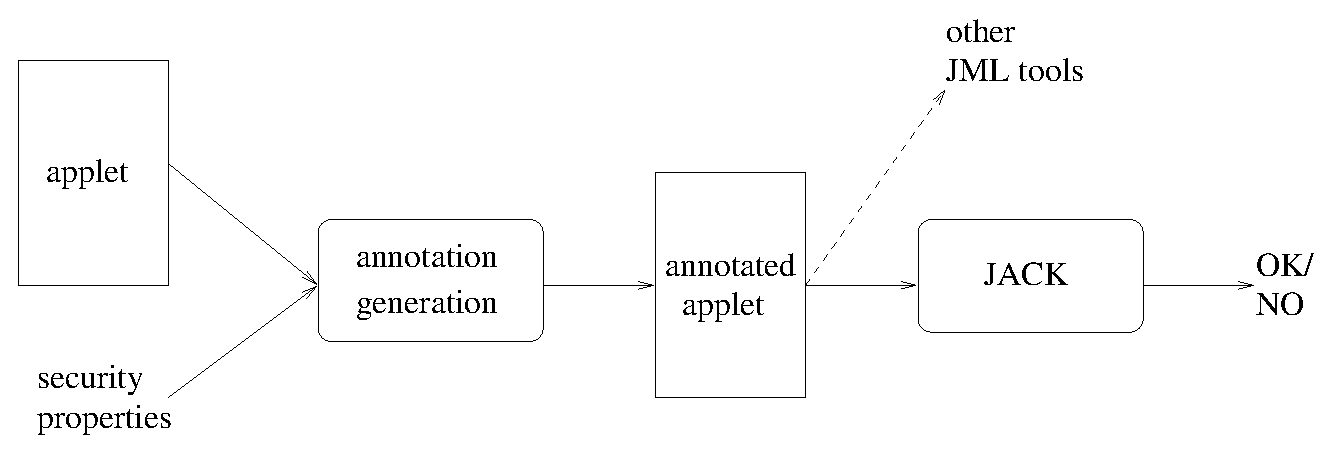
\epsfig{file=isaac.eps, width=9cm}
\end{center}
\caption{\sc Tool set for verifying high-level security properties}\label{FigArch}
\end{figure}



Figure~\ref{FigArch} shows the general architecture of the tool set
for verifying high-level security properties. Our annotation generator
can be used as a front-end for any tool accepting JML-annotated Java
(Card) applications. As input we have a security property and a Java
Card applet. The output is a JML Abstract Syntax Tree (AST), using the
format as defined for the standard JML parser. When pretty-printed,
this AST corresponds to a JML-annotated Java file. From this
annotated file, JACK generates appropriate proof obligations to check
whether the applet respects the security property.

\paragraph*{Automatic Generation of Annotations}
The purpose of this section is to provide a brief description of the
weaving phase, \emph{i.e.}~how the core-annotations are propagated
throughout the applet. We define functions \textsf{mod}, \textsf{pre},
\textsf{post} and \textsf{exc\-post}, propagating assignable clauses,
preconditions, postconditions and exceptional postconditions,
respectively. These functions have been defined and implemented for
the full Java Card language, but to present our ideas, we only give
the definitions for a representative subset of statements: statement
composition, method calls, conditional and \texttt{try}-\texttt{catch}
statements and special set-annotations. We assume the existence of
domains \textsf{MethName} of method names, \textsf{Stmt} of Java Card
statements, \textsf{Expr} of Java Card expressions, and \textsf{Var}
of static ghost variables, and functions \textsf{call} and
\textsf{body}, denoting a method call and body, respectively.

All functions are defined as mutual recursive functions on method
names, statements and expressions. When a method call is encountered,
the implementation will check whether annotations already have been
generated for this method (either by synthesizing or weaving). If not
it will recursively generate appropriate annotations. Java Card
applets typically do not contain (mutually) recursive method calls,
therefore this does not cause any problems. Generating appropriate
annotations for recursive methods would require more care (and in
general it might not be possible to do without any user interaction).


\paragraph{Propagation of assignable clauses}
First we define a function \textsf{mod} that propagates
assignable clauses for static ghost variables.

%Different from the standard JML set of modified variables in a method, that takes into account  both JML and 
%Java variables, we keep track only of JML ghost static variables. For our purposes this is sufficient because the generated pre- and postconditions involve only ghost variables.
\begin{definition}[\textsf{mod}]We define functions
%\[
%\begin{array}{rcl}
\(\mathsf{mod} \colon \mathsf{MethName} \rightarrow
\mathcal{P}(\mathsf{Var})\), 
\(
\mathsf{mod}  \colon  \mathsf{Stmt}   \rightarrow
\mathcal{P}(\mathsf{Var}) \), and 
\(\mathsf{mod}  \colon  \mathsf{Expr}   \rightarrow  \mathcal{P}(\mathsf{Var})\)
%\end{array}
%\]
by rules like (where \(m,n\,\colon\mathsf{MethName}\),
\(s_1,s_2\,\colon\mathsf{Stmt}\), \(c\,\colon\mathsf{Expr}\) and \(x\colon\mathsf{Var}\)):
\[
\begin{array}{rcl}
\mathsf{mod}(m) & = & \mathsf{mod}(\mathsf{body}(m)) \smallskip \\
\mathsf{mod}(s_1 \mathtt{;} s_2) & = & \mathsf{mod}(s_1) \cup \mathsf{mod}(s_2)\\
\mathsf{mod}(\mathsf{call}(n)) & = &  \mathsf{mod}(n) \\
\mathsf{mod}(\mathtt{if\:(} c \mathtt{)\:} s_1 \mathtt{\:else\:} s_2)
&=& \mathsf{mod}(c) \cup \mathsf{mod}(s_1) \cup \mathsf{mod}(s_2)\\
\mathsf{mod}(\mathtt{try\:} s_1 \mathtt{\:catch\:(} E \mathtt{)\:}
s_2) & = & \mathsf{mod}(s_1) \cup \mathsf{mod}(s_2)\\
\mathsf{mod}(\mathtt{set\:}x \mathtt{\:=\:} c) & = &  \{ x \} 
\end{array}
\]
\end{definition}


\paragraph{Propagation of preconditions}
Next, we define a function \textsf{pre} for
propagating preconditions. This function analyses a
method body in a sequential way---from beginning to end---computing
which preconditions of the methods called within the body have to be
propagated. To understand the reasoning behind the definition, we will
first look at an example. Suppose we are checking the \textbf{No
nested transactions} property for an application, which contains a
method \texttt{m}, whose only method calls are those shown, and which
does not contain any set annotations.
\begin{verbatim}
void m() { ... // some internal computations
           JCSystem.beginTransaction();
           ... // computations within transaction
           JCSystem.commitTransaction(); }
\end{verbatim}
Core-annotations are synthesised for \texttt{beginTransaction}
and \texttt{commit\-Transaction}. The annotations for
\texttt{beginTransaction} are shown below
\begin{verbatim}
/*@ requires TRANS == 0;
  @ assignable TRANS;
  @ ensures TRANS == 1; @*/
public static native void beginTransaction() 
                          throws TransactionException;
\end{verbatim}
Since the method is native, one cannot describe its body. However, if
it had been non-native, an annotation \texttt{//@ set TRANS = 1;}
would have been generated, to ensure that the method satisfies its
specification.

Likewise \texttt{commitTransaction} requires \texttt{TRANS == 1}
and ensures \texttt{TRANS == 0}. As we assume that \texttt{TRANS} is
not modified by the code that precedes the call to
\texttt{beginTransaction},  the only way the precondition of this method
can hold, is by requiring that it already holds at the moment
\texttt{m} is called. Thus, the precondition of
\texttt{beginTransaction} has to be propagated. In contrast, the
precondition for \texttt{commitTransaction} (\texttt{TRANS == 1})
has to be established by the postcondition of
\texttt{begin\-Transaction}, because the variable \texttt{TRANS} is
modified by this method. %Propagating the precondition of
%\texttt{commit\-Transaction} to the precondition of \texttt{m} would
%not help to guarantee that the precondition of
%\texttt{commitTransaction} holds. 
Thus, preconditions containing only unmodified variables should be
propagated.  Propagating pre- or postconditions can be considered as
passing on a method contract. Method bodies can only pass on contracts
for variables they do not modify; once they modify a variable it is
their duty to ensure that the necessary conditions are satisfied.

%In the definition of the function \textsf{pre} for propagating
%preconditions, we assume the existence of a function \textsf{mod}
%returning the set of static ghost variables modified by a
%statement. 
%As we are only interested in static ghost variables with
%primitive types, the definition is straightforward and it does not
%have to consider aliasing. 

We assume the existence of a domain \textsf{Pred} of predicates using
static ghost variables only, and function
\textsf{fv}, returning the set of free variables.

%We define \textsf{pre} on method names, statements and
%expressions. These definitions are mutually recursive.  Java Card
%applets typically do not contain (mutually) recursive method calls,
%therefore this does not cause any problems. Generating appropriate
%annotations for recursive methods would require more care (and in
%general it might not be possible to do without any user interaction).
%\begin{definition} [\textsf{pre\_init}]
%\[
%\begin{array}{rcl}
%\mathsf{pre\_init}& \colon & \mathsf{MethName} \rightarrow  \mathcal{P}(\mathsf{Pred})
%\end{array}
%\]
%\end{definition}
%The function $\textsf{pre\_init}$ returns the predicate that a method declaration is initialised with. Such an initialisation can be seen 
%for example as the specification added for the  ``core'' methods. It is in fact any pre- or postcondition specified for a method before applying the functions that  we define.  
\begin{definition}[\textsf{pre}]
We define
%\[
%\begin{array}{rcl}
\(\mathsf{pre} \colon \mathsf{MethName} \rightarrow
\mathcal{P}(\mathsf{Pred})\),
\( \mathsf{pre}  \colon  \mathsf{Stmt} \rightarrow
\mathcal{P}(\mathsf{Var}) \rightarrow \mathcal{P}(\mathsf{Pred}) \), and
\( \mathsf{pre}  \colon  \mathsf{Expr} \rightarrow
\mathcal{P}(\mathsf{Var}) \rightarrow \mathcal{P}(\mathsf{Pred}) \)
%\end{array}
%\]
by rules like (where \(m,n\,\colon\mathsf{MethName}\),
\(s_1,s_2\,\colon\mathsf{Stmt}\), \(c\,\colon\mathsf{Expr}\),
\(V\colon\mathcal{P}(\mathsf{Var})\) and \(x\colon\mathsf{Var}\)): 
\[
\begin{array}{rcl}
\mathsf{pre}(m) & = & \mathsf{pre}(\mathsf{body}(m), \emptyset) \smallskip\\
\mathsf{pre}(s_1 \mathtt{;} s_2, V) & = & \mathsf{pre}(s_1, V) \cup 
                                          \mathsf{pre}(s_2, V \cup \mathsf{mod}(s_1))\\

\mathsf{pre}(\mathsf{call}(n),V) & = & 
                \{ p \mid p \in \mathsf{pre}(n) \wedge 
                          (\mathsf{fv}(p) \cap V) = \emptyset\}\\
\mathsf{pre}(\mathtt{if\:(} c \mathtt{)\:} s_1 \mathtt{\:else\:} s_2, V) & = &
   \mathsf{pre}(c, V) \cup 
   \mathsf{pre}(s_1, V \cup \mathsf{mod}(c)) \cup\\
&&   \mathsf{pre}(s_2, V \cup \mathsf{mod}(c))\\
\mathsf{pre}(\mathtt{try\:} s_1 \mathtt{\:catch\:(} E \mathtt{)\:} s_2, V) & = & 
   \mathsf{pre}(s_1, V) \cup 
   \mathsf{pre}(s_2, V \cup \mathsf{mod}(s1))\\
\mathsf{pre}( \mathtt{set\:} x \mathtt{\:=\:} c) & = & \{\: \}
\end{array}
\]
\end{definition}

In the rules defining \textsf{pre} on \textsf{Stmt} and \textsf{Expr},
the second argument denotes the set of static ghost variables that have been
modified so far. When calculating the precondition for a method, we
calculate the precondition of its body, assuming that so far no variables
have been modified. For a statement composition, we first
propagate the preconditions for the first sub-statement, and then for
the second sub-statement, but taking into account the variables
modified by the first sub-statement. When propagating the preconditions
for a method call, we propagate all preconditions of the called method
that do not contain modified variables.  Since we are restricting our
annotations to expressions containing static ghost variables only, in
the rule for the conditional statement we cannot take the outcome of
the conditional expression into account. As a consequence, we
sometimes generate too strong annotations, but in practice this does
not cause problems. Moreover, it should be emphasised that this
only can make us reject correct applets, but it will never make us
accept incorrect ones.  Similarly, for the
\texttt{try}-\texttt{catch} statement, we always propagate the
precondition for the \texttt{catch} clause, without checking whether it
actually can get executed. Again, this will only make us reject
correct applets, but it will never make us accept incorrect
ones. Finally, a set annotation does not give rise to any propagated
precondition. 

Notice that by definition, we have the following property for the
function \textsf{pre} (where \(s\) is either in \textsf{Stmt} or
\textsf{Expr}, and \(V\) is a set of static ghost variables).
\[
p \in \textsf{pre}(s, V) \Leftrightarrow (p \in \textsf{pre}(s,
\emptyset) \wedge (\textsf{fv}(p) \cap V) = \emptyset)
\]

\paragraph{Propagation of postconditions}
In a similar way, we define functions \textsf{post} and
\textsf{exc\-post},  computing the
set of postconditions and exceptional postconditions that have to be
propagated for method names, statements and expressions. The main
difference with the definition of \textsf{pre} is that these functions run
through a method from the end to the beginning. Moreover, they have to
take into account the different paths through the method. For
each of these possible paths, we calculate the appropriate
(exceptional) postcondition. The overall (exceptional) postcondition
is then defined as the disjunction of the postconditions related to
the different paths through the method. 

\paragraph{Example}
For the example discussed above, our functions compute the following
annotations.

\begin{verbatim}
/*@ requires TRANS == 0;
  @ assignable TRANS;
  @ ensures TRANS == 0; @*/
void m() { 
   ... // some internal computations
  JCSystem.beginTransaction();
  ... // computations within transaction
  JCSystem.commitTransaction(); }
\end{verbatim}
This might seem trivial, but it is important to realise that similar
annotations will be generated for all methods calling
\texttt{m}, and transitively for all methods calling the methods
calling \texttt{m} \emph{etc.}
Having an algorithm to generate such annotations enables to check
automatically a large class of high-level security properties.


\subsection{Bytecode validation}
An objective of the Inspired project is to develop tools allowing to built secure framework for post-issued applications. The bytecode verification framework embedded in JACK is the way to support this feature.  

We propose a bytecode verification framework with the following components: a bytecode specification language, a compiler from source
 program annotations into bytecode annotations and a verification condition generator over Java bytecode.

In a client-producer scenario, these features bring to the producer means to supply the sufficient specification information 
which will allow the client to establish trust in the code, especially when the client policy is potentially complex and a fully automatic specification inference
will fail. On the other hand, the client is supplied with a procedure to check the untrusted annotated code. 

  

Our approach is tailored to Java bytecode.
The Java technology is widely applied to mobile and embedded components because of its portability across platforms. 
For instance, its dialect JavaCard is largely used in smart card applications and the J2ME Mobile Information Device Profile 
(MIDP) finds application in GSM mobile components. 
%In this article, we propose a static verification technique using formal methods for sequential Java bytecode programs.

The proposed scheme is composed of several components.
 We define a bytecode specification language, called BML, and supply a compiler from 
 the high level Java specification language JML~\cite{JMLRefMan} to BML. 
 BML supports a JML subset which is expressive enough to specify rich functional properties. 
The specification is inserted in the class file format in newly defined attributes and thus makes not
 only the code mobile but also its specification. These class
 file extensions do not affect the JVM performance.
We define a bytecode logic in terms of weakest precondition calculus for the sequential Java bytecode language. 
The logic gives rules for almost all Java bytecode instructions and supports the Java specific features such as
exceptions, references, method calls and subroutines.  
 We have implementations of a verification condition generator based on the weakest precondition calculus and of
 the JML specification compiler. Both are part of JACK.

  The full specifications of the JML compiler, the weakest precondition predicate transformer definition and its proof of correctness can be found in~\cite{JBL05MP}.
  
The remainder of this section is organized as follows: 
Subsection~\ref{architecture_s} reviews scenarios in which the architecture may be appropriate to use; 
 Subsection~\ref{bcSpecLg} presents the bytecode specification language BML and the JML compiler; Subsection~\ref{wpbc} discusses the main
features of the \wpi (short for weakest precondition calculus); Subsection~\ref{pogEquiv} discusses the relationship between the verification conditions for JML annotated source and BML annotated bytecode.


\subsubsection{Applications}
\label{architecture_s}  


The overall objective is to allow a client to trust a code produced by an untrusted code producer. Our approach is especially suitable
 in cases where the client policy involves non trivial functional or safety requirements and thus, a full automatization of the verification 
process is impossible. To this end, we propose a PCC technique that exploits the JML compiler and the weakest predicate function presented in the article. 
 
 The framework is presented in Fig.~\ref{architecture}; note that certificates and their checking are not yet implemented
 and thus are in oblique font.
  


 \begin{figure}[!tbp]
 \centering
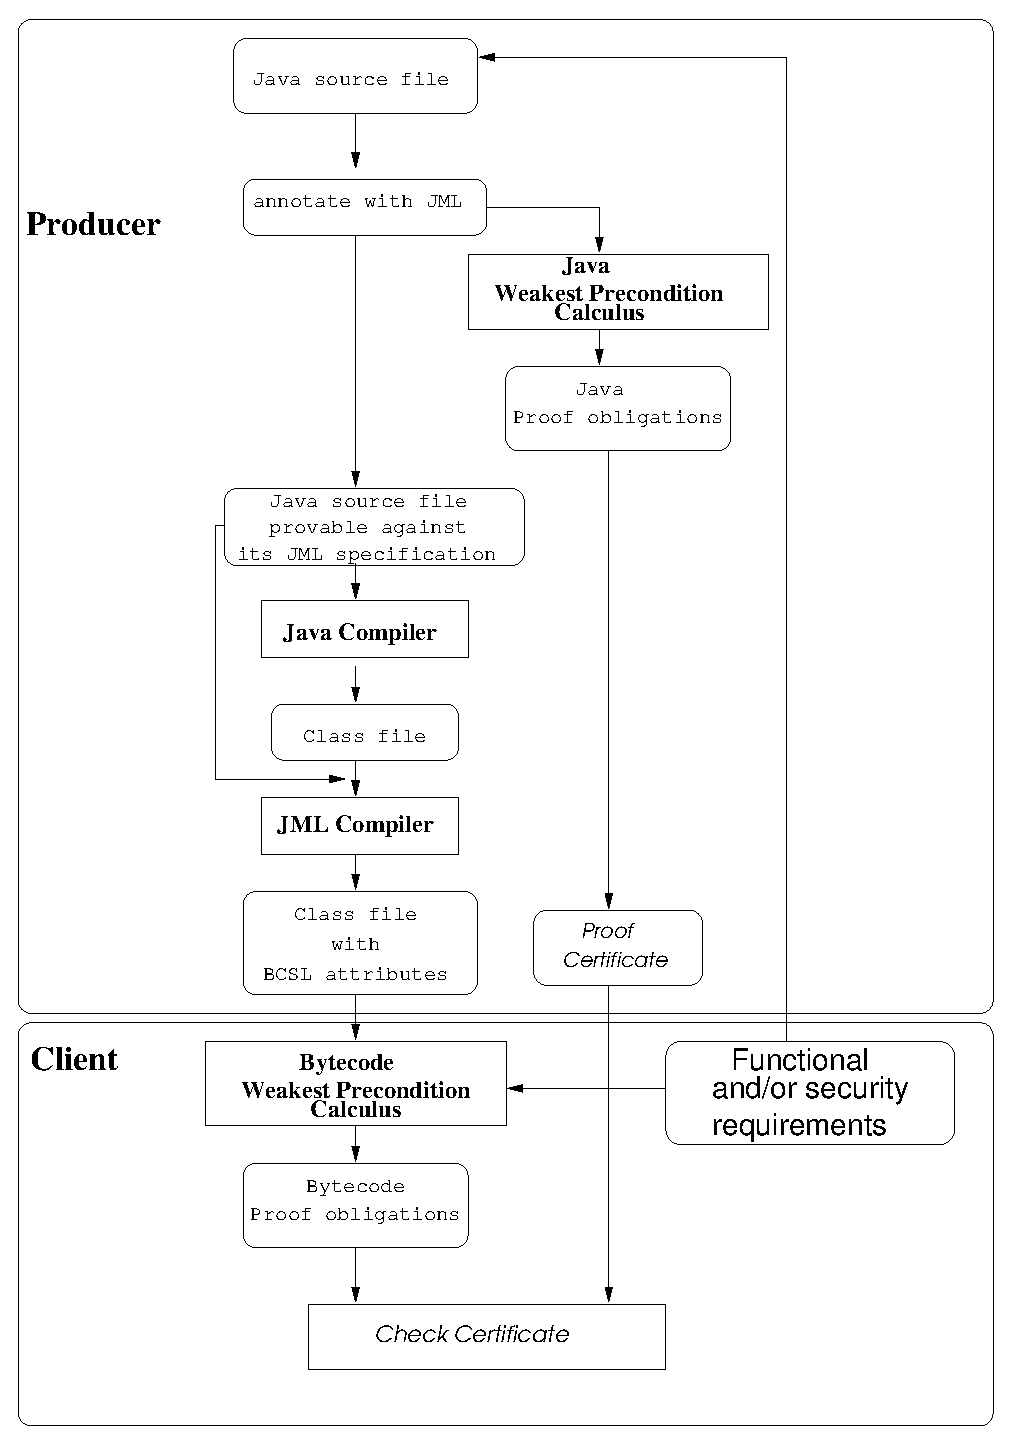
\epsfig{ file=sac.eps, width=10cm}
\caption{\sc The overall architecture for client producer scenarios }
\label{architecture}
\end{figure}

In the first stage of the process the client provides the functional
and (or) security requirements to the producer.  The requirements can
be in different form:
\begin{itemize}
\item Typical functional requirements can be a specified interface
describing the application to be developed. In that case, the client
specifies in JML the features that have to be implemented by the code
producer.
\item Client security requirements can be a restricted access to some
method from the API expressed as a finite state machine.  For example,
suppose that the client API provides transaction management facilities
- the API method \texttt{open} for opening and method \texttt{close}
for closing transactions. In this case, a requirement can be for no
nested transactions.  This means that the methods \texttt{open} and
\texttt{close} can be annotated to ensure that the method
\texttt{close} should not be called if there is no transaction running
and the method \texttt{open} should not be called if there is already
a running transaction. In this scenario, we can apply results of
previous work \cite{m+04:cardis}.  
\end{itemize}
Usually, the development process involves annotating the source code
with JML specification, generating verification conditions, using
proof obligation generator over the source code and discharging proofs
which represent the program safety certificate and finally, the
producer sends the certificate to the client along with the annotated
class files.  Yielding certificates over the source code is based on
the observation that proof obligations on the source code and
non-optimized bytecode respectively are syntactically the same modulo
names and basic types. Every Java file of the untrusted code is
normally compiled with a Java compiler to obtain a class file. Every
class file is extended with user defined attributes that contain the
BML specification, resulting from the compilation of the JML
specification of the corresponding Java source file.


We have extended the Jack tool with a compiler from
 JML to BML and a bytecode verification condition generator. In the next sections, we introduce
 the BML language, the JML compiler and the bytecode \wpi calculus which underlines the bytecode verification condition generator.
 

\subsubsection{Bytecode Specification Language}\label{bcSpecLg}

In this section, we introduce a bytecode specification language which we call BML (short for ByteCode Specification Language).
 BML is based on the design principles of JML (Java Modeling Language)~\cite{JMLRefMan}, which is a behavioral interface specification 
language following the design by contract approach \cite{M97oos}.

In the following, we give the grammar of BML and sketch the compiler from JML to BML. 

\paragraph{Grammar} \label{grammar}


BML corresponds to a representative subset of JML and is expressive enough for most purposes including the description of non trivial functional and security properties.


 Specification clauses in BML that are taken from JML and inherit their semantics directly from JML include:
class specification, i.e. class invariants and history constraints, 
  method preconditions, normal and exceptional postconditions, method frame conditions (the locations that may be modified by the method), inter method specification, as for instance loop invariants and loop frame conditions(this is not a standard feature of JML but we were inspired for this by the JML extensions in JACK ~\cite{BRL-JACK}). 
We also support specification inheritance and thus behavioral subtyping as described in \cite{Dhara-Leavens96}. Most of the Java expressions like field access expressions, local variables, etc can be mentioned in the BML specification.
BML supports the standard JML specification operators as for example, $\old{\expression}$ which is used in method postconditions and
 designates the value of the expression $\expression$ in the prestate of a method, $ \result$ which stands for the value the method
returns if it is not void,  $\typeof{\expression}$ which stands for type of $\expression$ etc.  

\subsubsection{Compiling JML into BML}\label{comJML}


We now turn to explaining how JML specifications are compiled into user defined attributes for Java class files. Recall that a class file defines
a single class or interface and contains information about  the class name, interfaces implemented by the class, super class, methods and fields declared in the class and references. The Java Virtual Machine Specification (JVM) \cite{VMSpec} mandates that the class file contains data structure usually referred as the \textbf{constant\_pool} table which is used to construct the runtime constant pool upon class or interface creation. The runtime constant pool serves for loading, linking and resolution of references used in the class. The JVM allows to add to the class file user specific information(\cite{VMSpec}, ch.4.7.1). This is done by defining user specific attributes  (their structure is predefined by JVM).

Thus the ``JML compiler'' \footnote{not to be confused, Gary Leavens also calls his tool jmlc JML compiler, which transforms JML into runtime checks and thus generates input for the jmlrac tool  } compiles the JML source specification into user defined attributes. The compilation process has three stages:
\begin{enumerate}
\item Compilation of the Java source file. This can be done by any Java compiler that supplies for every method in the generated class file 
the \textbf{Line\_Number\_Table} and \textbf{Local\_Variable\_Table}  attributes. The presence in the Java class file format of 
these attribute is optional \cite{VMSpec}, yet almost all standard non optimizing compilers can generate these data. 
The \textbf{Line\_Number\_Table} describes the link between the source line and the bytecode of a method.  
The \textbf{Local\_Variable\_Table} describes the local variables that appear in a method. 
Those attributes are important for the next phase of the JML compilation.
\item Compilation of the JML specification from the source file and the resulting class file. In this phase, Java and JML source identifiers are 
linked with their identifiers on bytecode level, namely with the corresponding indexes either from the cp (short for constant pool) or the array of 
local variables described in the \textbf{Local\_Variable\_Table} attribute. If a field
identifier, for which no cp index exists, appears in the JML specification, a new index is added in the cp and the field identifier in question
is compiled to the new cp index. It is also in this phase that the specification parts like the loop invariants and the assertions which should hold at a certain point in the source program must be associated to the respective program point on bytecode level. The specification
is compiled in binary form using tags in the standard way. The compilation of an expression is a tag followed by the compilation of its subexpressions. 

Another interesting point in this stage of the JML compilation is how the type differences on source and bytecode level are treated. 
The JVM does not provide a direct support for integral types like byte, short, char, neither for boolean.
 Those types are rather encoded as integers in the bytecode. The JML compiler performs transformation on specifications that involve Java boolean values and variables.
% We illustrate this by an example in Fig.~\ref{postCompile}, which shows the resulting compilation of the postcondition of method \texttt{isElem} in Fig.~\ref{replaceSrc}. The example also shows that local variables and  fields are respectively linked to the index of the register table for the method and to the corresponding index of the cp table  (\#19 is the compilation of the field name \texttt{list} and \register{1} stands for the method parameter \texttt{obj}). 


\item add the result of the compiled specifications components in
newly defined attributes in the class file.
 For example, the specifications of all the loops in a method are compiled to a unique method attribute whose syntax is given in Fig.~\ref{loopAttribute}. This attribute is an array of data structures each describing a single loop from the method source code. 
More precisely, every element contains information about the instruction where the loop starts as specified in the
\textbf{Line\_Number\_Table}, the locations that can be modified in a loop iteration, 
 the invariant associated to this loop and the decreasing expression in case of total correctness, 

\end{enumerate}

\begin{figure}[htp]
\textbf{
\begin{tabbing}
JML\=Loop\_specification\_attribute \{ \\
\> ...\\
\> \{\hspace{3 mm}\=  index;\\
\> \>  modifies\_count;\\
\> \> formula modifies[modifies\_count];\\
\> \> formula invariant;\\
\> \> expression decreases;\\
\> \} loop[loop\_count];\\
\}
\end{tabbing}
}

\caption{\sc Structure of the loop specification attribute}
\label{loopAttribute}

\end{figure}
 The most problematic part of the specification compilation is the identification of
 which loop in the source corresponds to which bytecode loop in the control flow
 graph. To do this, we assume that the control flow graph is reducible, 
i.e. there are no jumps into the middle of the loops from outside; graph reducibility allows to establish the same order between loops in the
 bytecode and source code level and to find the right places in the bytecode where the loop invariants must hold.


\subsubsection{Weakest Precondition Calculus For Java
Bytecode}\label{wpbc} In this section, we define a bytecode logic in
terms of a weakest precondition calculus. The proposed weakest
precondition \wpi \ supports all Java bytecode sequential instructions
except for floating point arithmetic instructions and 64 bit data
(\java{long} and \java{double} types), including exceptions, object
creation, references and subroutines. The calculus is defined over the
method control flow graph and supports BML annotation, i.e. bytecode
method's specification like preconditions, normal and exceptional
postconditions, class invariants, assertions at particular program
point among which loop invariants. The verification condition
generator applied to a method bytecode generates a proof obligation
for every execution path by applying first the weakest predicate
transformer to every \instr{return} instruction, \instr{athrow}
instruction and end of a loop instruction and then following in a
backwards direction the control flow up to reaching the entry point
instruction. In a related document \cite{JBL05MP}, we show that the
$\wpi$ function is correct.


 In Fig.~\ref{instrWP}, we show the \wpi \ rule for the \instr{Type\_load i} instruction.
 As the example shows the \wpi \ function takes three arguments:
the instruction for which we calculate the precondition, 
the instruction's postcondition $\psi$ and the exceptional postcondition function $\excPost$ which for any exception \texttt{Exc} and 
instruction index \texttt{ind} returns the
corresponding exceptional postcondition $\excPost(\texttt{Exc}, \tt{ind})$. One can also notice that the rule involves the stack expressions \counter 
(stands for the counter of the method execution stack) \ and \stack{ i } (stands for the element at ind \texttt{i} from the stack top).
 This is because the JVM is stack based and the instructions take their arguments from the method execution stack and 
 put the result on the stack.
 The \wpi \ rule for  \instr{Type\_load i} increments the stack counter \counter \ and loads on the stack top the contents
 of the local variable $\register{i}$. 




\begin{figure}[htp]
\[
\begin{array}{l}
\wpi(\instr{Type\_load \ i}, \ \psi, \ \excPost)  = \\
\begin{array}{l}  \psi\substitution{\counter }{\counter+1} \substitution{\stack{\counter+1}}{\register{i}} \end{array} \\
\\
\\
 \wpi(\instr{putField} \ \texttt{Cl.f}, \ \psi, \ \excPost)  = \\
\begin{array}{l}
                \stack{\counter -1} \not= \Mynull\Rightarrow   
         \psi\begin{array}{l} \substitution{\counter}{ \counter-2 } \\[0 mm] 
                           \substitution{\texttt{Cl.f} }{ \texttt{Cl.f}\oplus [\stack{\counter -1} \rightarrow \stack{\counter}] } \\
                \end{array}\\

   \wedge \\
        \stack{\counter-1} = \Mynull    \Rightarrow \excPost(\tt{NullPointerExc})
        \begin{array}{l}
          \substitution{ \counter }{ 0} \\
          \substitution{\stack{0}}{ \stack{\counter}} 
        \end{array}
    \end{array} %\biggr. & \\
\end{array}
 \]       
\caption{\sc Examples for bytecode wp rules}
 \label{instrWP}

\end{figure}

In the following, we consider how instance fields, %method invocations, 
loops exception handling and subroutines are treated. We omit here aspects like method invocation and object creation because of space limitations but a detailed explanation can be found in~\cite{JBL05MP}. 

\subparagraph*{Manipulating object fields}
Instance fields are treated as functions, where the domain of a field \texttt{f} 
declared in the class \texttt{Cl} is the set of objects of class \texttt{Cl} and its subclasses.
We are using function updates when assigning a value to a field reference as, for instance in~\cite{B00ppp}.
In Fig.\ref{instrWP}, we give the \wpi \ rule for the
instruction \instr{putfield} \texttt{Cl.f}, which updates the field \texttt{Cl.f}\footnote{ \texttt{Cl.f} stands for the field \texttt{f} declared in class 
\texttt{Cl}} of the object referenced by the reference stored in the stack below the stack top \stack{\counter-1} with the value on the stack top \stack{\counter}.
Note that the rule takes in account the possible exceptional termination of the instruction execution.


\subparagraph*{Loops}

Identifying loops on bytecode and source programs is different because of their different nature --- 
the first one lacks while the second has structure. While on source level loops correspond to loop statements,  
on bytecode level we have to analyze the control flow graph in order to find them.
 The analysis consists in looking for the backedges in the control flow graph using standard compiler techniques. 
  
 We assume that a method's bytecode is provided with sufficient specification and in particular loop invariants.
 Under this assumption, we build an abstract control flow graph where the backedges are replaced by
 the corresponding invariant. We apply the \wpi \ function over the abstract version of the control flow graph which generates verification conditions for the 
preservation and initialization of every invariant in the abstraction graph. 


     

\subparagraph*{Exceptions and Subroutines}
Exception handlers are treated by identifying the instruction at which the handler compilation starts. The JVM specification mandates 
that a Java compiler must supply for every method an \textbf{Exception\_Table} attribute that contains data structures describing the compilation of every implicit (in the presence of subroutines) or explicit exception handler: the instruction at which the compiled exception handler starts,
 the protected region (its start and end instruction indexes), and the exception type the exception handler protects from. Thus, 
for every instruction \instr{ins} in method \method~ which may terminate exceptionally on exception \texttt{Exc} the exceptional function
 $\excPost$  returns the \wpi \ predicate of the exceptional handler protecting \instr{ins} from \texttt{Exc} if such a handler exists.
Otherwise, $\excPost$ returns the specified exceptional postcondition for exception \texttt{Exc} as specified in the specification of
method \method.

Subroutines are treated by abstract inlining\footnote{NB: we do not transform the bytecode. It is rather the \wpi \
 function that treats subroutines as if the subroutines were inlined}. First, the instructions of every subroutine
 are identified. %To this end, we suppose that the bytecode has
% been certified by a bytecode verifier which guarantees
%that there are no recursive subroutines.
To this end, we assume that the code has passed the bytecode verification and that every subroutine terminates with a \instr{ret} 
instruction(usually, the compilation of subroutines ends with a \instr{ret} instruction but it is not always the case). Thus, by abstract inlining, we mean that
 whenever the \wpi~function is applied to an instruction \instr{jsr}  \texttt{ind}, a postcondition $\psi$ and an exceptional postcondition function $\excPost$, its precondition  $\wpi^{\instr{jsr} \ \tt{ind}}$ is calculated as follows: the \wpi \ is applied to the bytecode instructions that represent the subroutine which starts at instruction \texttt{ind},
 the postcondition $\psi$ and the exceptional postcondition function  $\excPost$.





 \subsubsection{Relation between verification conditions on source and
 bytecode level } \label{pogEquiv} 

In order to establish the validity of source level verification, we
must relate proof obligations at source level to proof obligations at
bytecode level. We have shown that compilation (almost) preserves
proof obligations, in the sense that the set of proof obligations
generated for an annotated source code program is equal to the set of
proof obligations generated for the corresponding annotated compiled
program. Formal developments may be found
in~\cite{gta05:fast,BP06:sac}.


At a pratical level, the relationship between the source code proof
obligations generated by the standard feature of JACK and the bytecode
proof obligations generated by our implementation over the
corresponding bytecode produced by a non optimizing compiler over the
examples given in \cite{JPVC03JKM}. The proof obligations were the
same modulo names and short, byte and boolean values as well as
hypothesis names. The proof obligations on bytecode and source level
that we proved interactively in Coq produced proof scripts which were
also equal modulo those values and the hypothesis's names. This means
that an appropriate encoding of proof obligations on source and
bytecode level can be found, where the names of the source and
bytecode hypothesis are the same and where the source obligations can
be transformed in such a way that the produced proof script for the
transformed source proof obligation can be applied to the
corresponding one on bytecode level. This shall be useful in future
scenarios for TPD with dynamic loading of program and components.





